\section{Software-Modellering}\label{softwaremodellering}

\subsection{Designklassediagram(DCD)}

På baggrund af objekt og domænemodellerne, se afsnit \ref{businessmodellering}, har vi udarbejdet en DCD, der skal hjælpe os med at give overblik over arkitekturen i programmet.

DCD'en er blevet opdateret mange gange siden den første udgave, der blev lavet inden vi startede med at kode.

Det har været en stor hjælp til at finde ud af, hvilke dele af programmet skal have hvilket ansvar.

Internt i gruppen har DCD'en også været meget omdiskuteret, da den har tydeliggjort de softwarearkitektokniske valg og minimeret interne misforståelser.


På figur \ref{fig:DCDMenu} kan DCD'en for vores 2 menu klasser, menu interfacet og controller klassen ses.
Vi har valgt at opbygge programmet således, at vi har menuer, der kender til en controller klasse.
Denne controller klasse forbinder med et timeregistreringsbibliotek, der indeholder alt logikken for vores timeregistreringssystem.

En DCD for timeregistreringsbiblioteket kan ses i på figur \ref{fig:DCDLib} på side \pageref{fig:DCDLib} i bilagene.

\begin{figure}[H]
    \makebox[\textwidth][c]{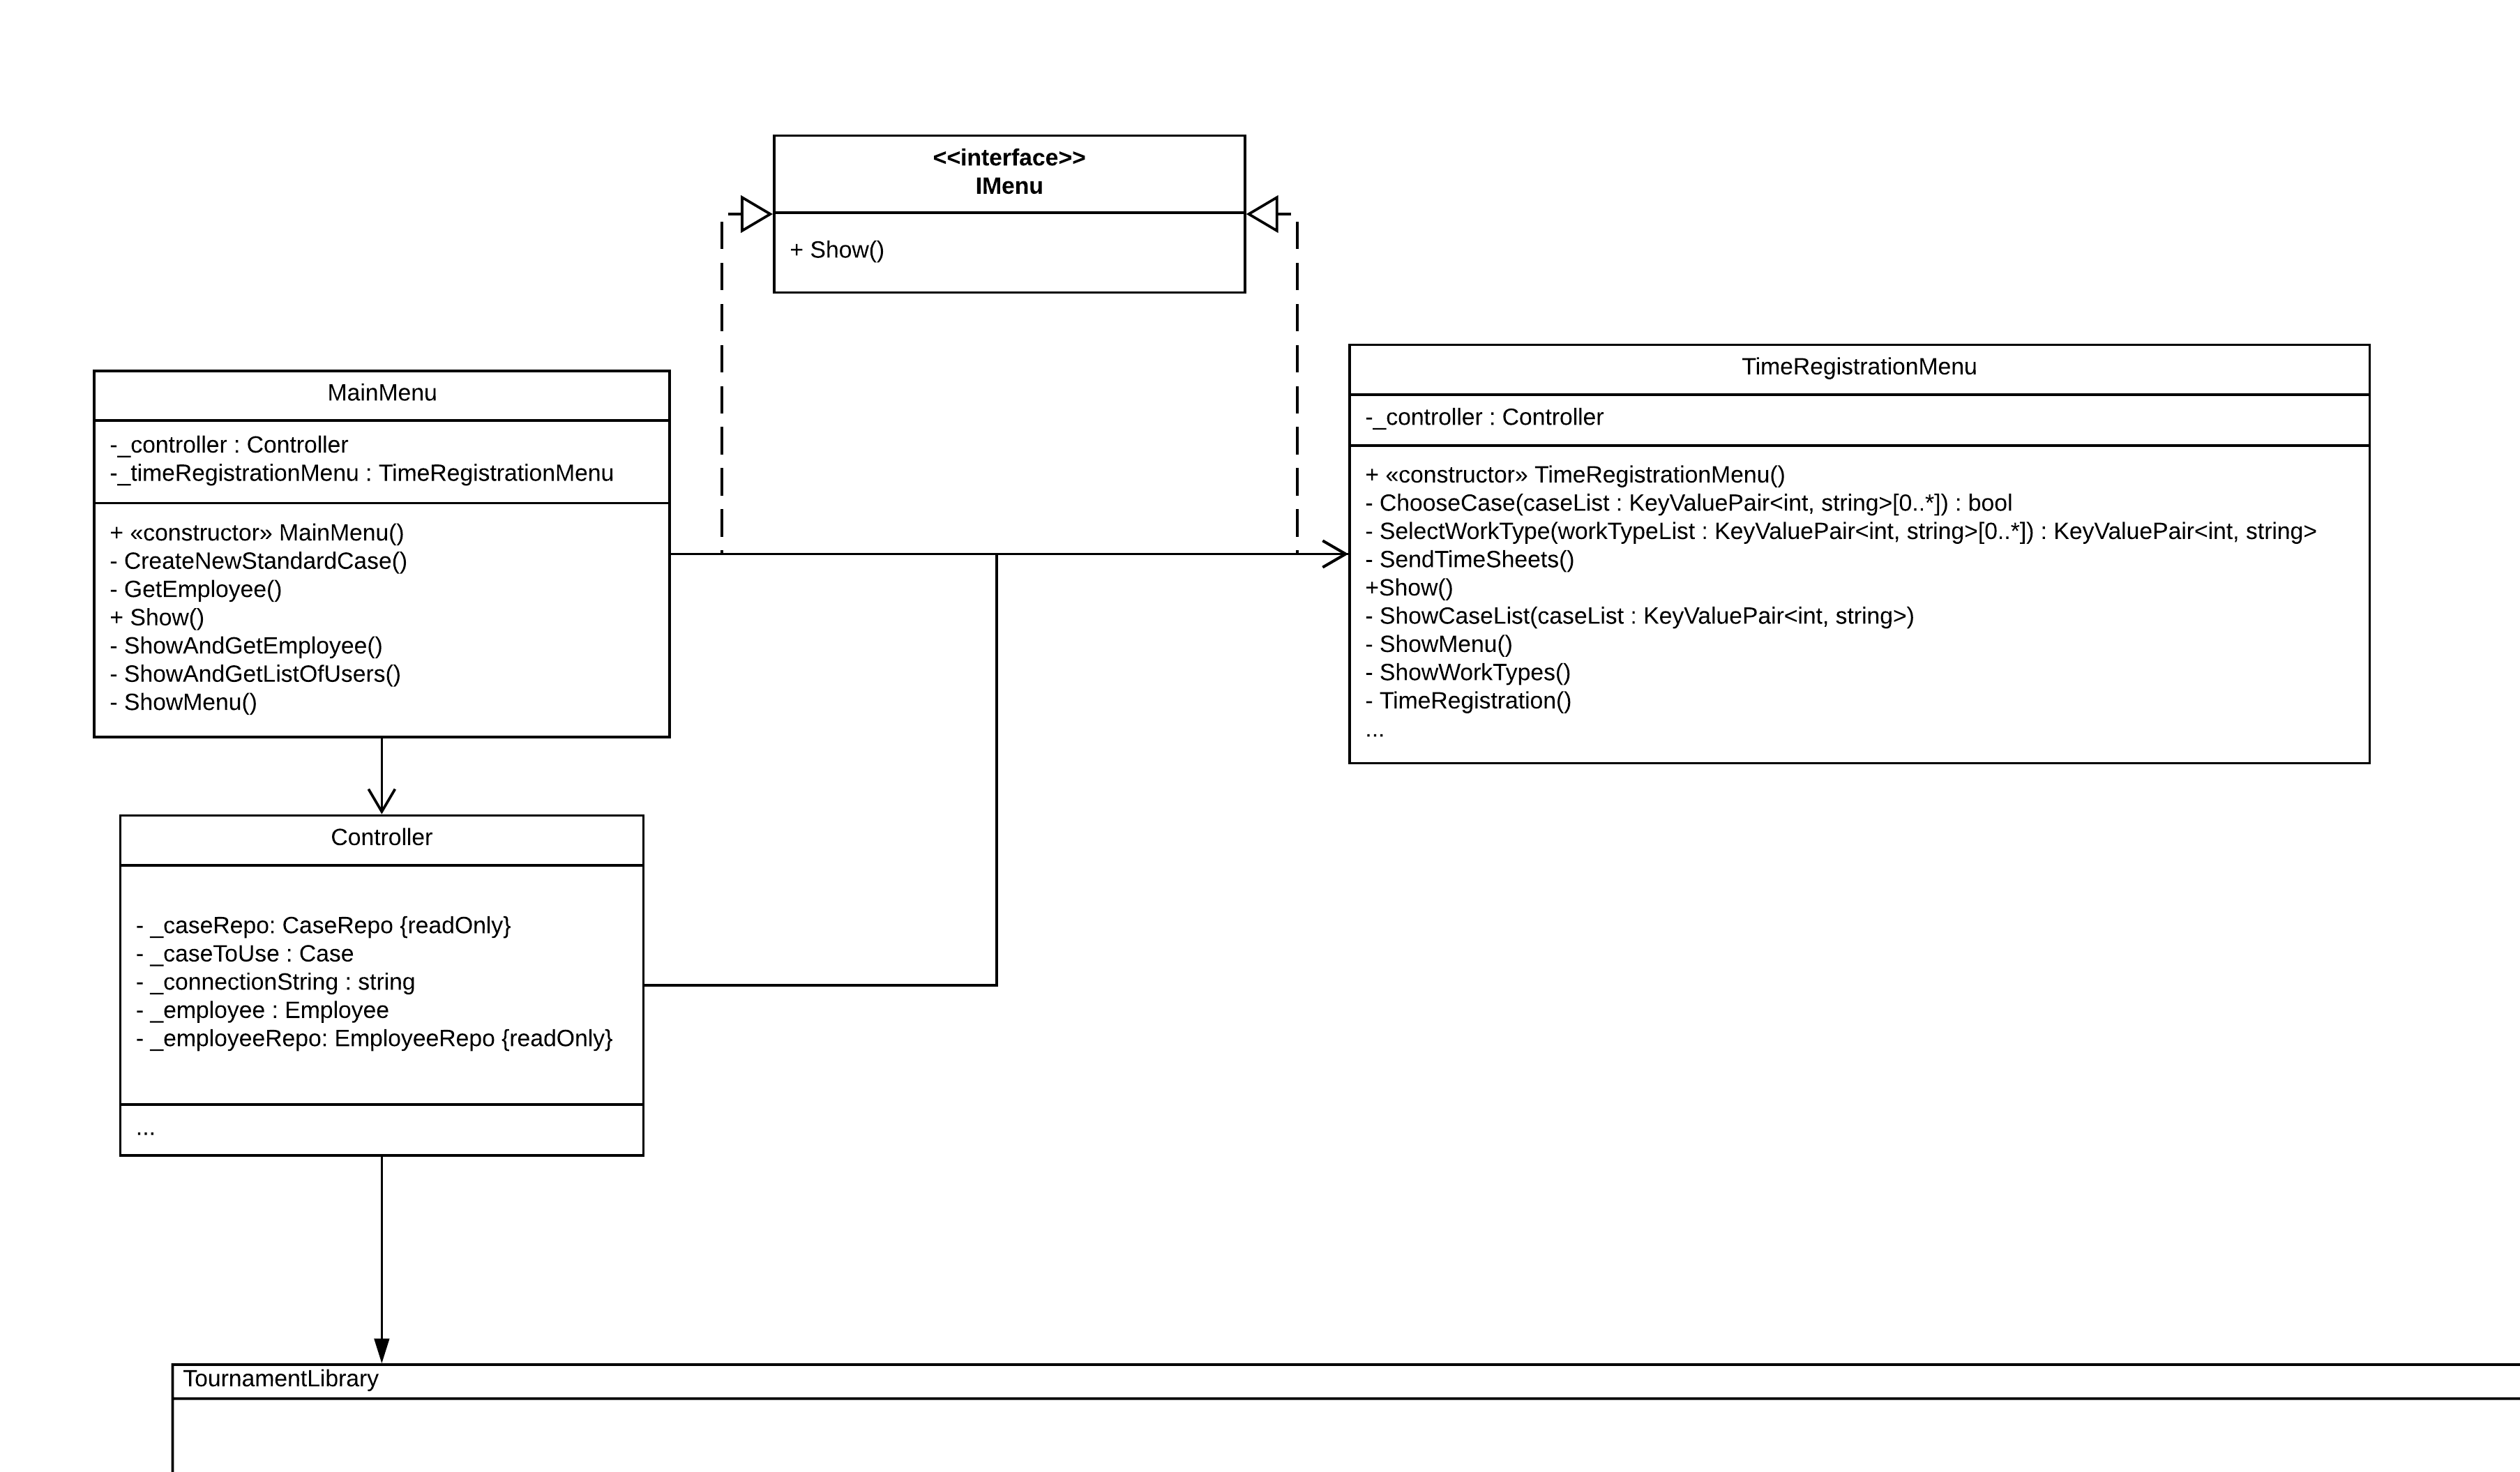
\includegraphics[scale = .6]{DCDMenu.png}}
    \caption{DCD for menu og controller klasser.}
    \label{fig:DCDMenu}
\end{figure}

\subsection{Systensekvensdiagram(SSD) modellering}

Ud fra use casen beskrevet i afsnit \ref{ssec:usecase} har vi lavet følgende systemsekvensdiagram, der beskriver, hvordan en tømrer skal bruge systemet. SSD'en kan ses på figur \ref{fig:SSDMain}.

Dette hjælper os med at forstå, hvordan systemet skal implementeres, blandt andet ved at specificere hvilke metoder, der får hvilke input fra brugeren.
\begin{figure}[H]
    \makebox[\textwidth][c]{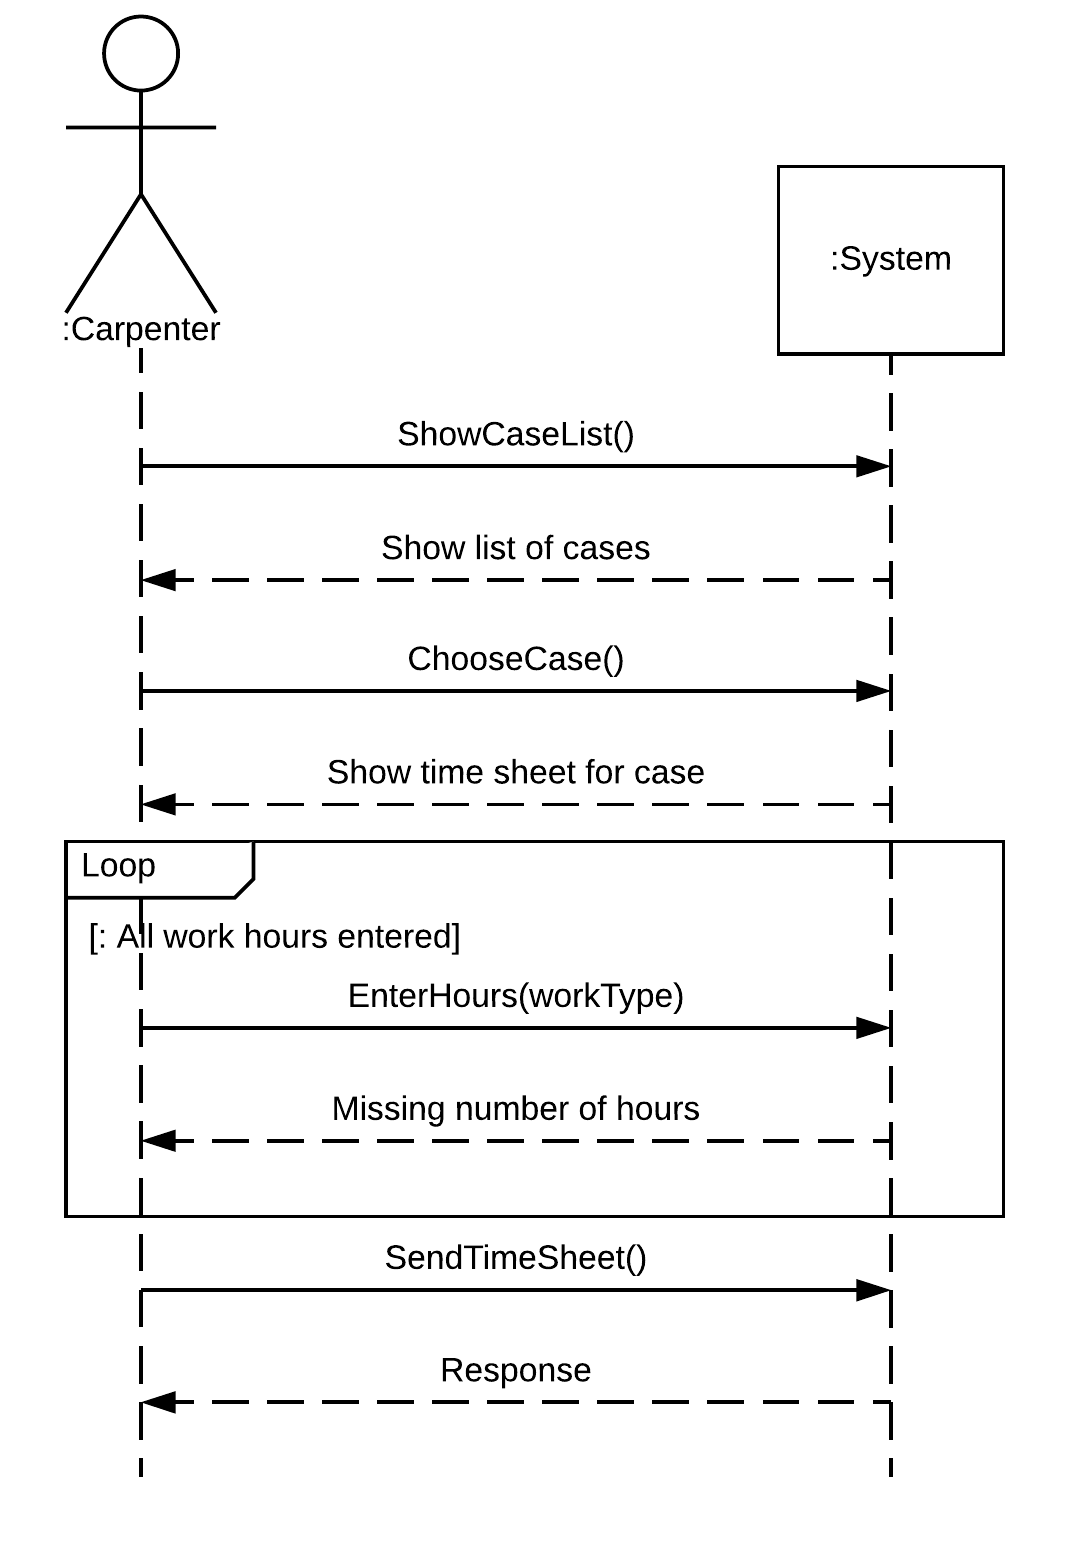
\includegraphics[scale = 1]{SSDMain.png}}
    \caption{DCD for menu og controller klasser.}
    \label{fig:SSDMain}
\end{figure}

\subsection{Softwareoperationskontrakt(SOC) modellering}

Det næste skridt for at gå fra virksomhedens problem til at kode en løsning er at lave en SOC, der beskriver, hvordan tilstandene i systemet ændrer sig, når det bruges.

For use casen \textbf{registrering af timer}, beskrevet i afsnit \ref{ssec:usecase} og SSD'en set på figur \ref{fig:SSDMain}, har vi udledt følgende SOC'er:

\textbf{Operation:} ShowcaseList()

\textbf{Cross Reference:} Use case: Registering af Timer.

\textbf{Pre condition:} Der findes en liste af cases.

\textbf{Post condition:}

\textbf{Output:} Listen vises.

Denne SOC har ingen post condition, da systemets tilstand ikke ændrer sig, men der blot vises en liste af cases.
Derfor har vi også tilføjet \textbf{output} parameteren, der beskriver, hvad der vises for brugeren.

For samme use case har vi også lavet følgende SOC:

\textbf{Operation:} EnterWorkHours(workType)

\textbf{Cross Reference:} Use case: Registering af Timer.

\textbf{Pre condition:} Der er blevet valgt en sag.

\textbf{Post condition:} Timer er blevet tilføjet til sagen.

Her kan det ses, at systemets tilstand skal ændres, da der skal tilføjes timer til den sag, der er valgt.

\subsection{Sekvensdiagram(SD) modellering}

Et godt værktøj til at visualisere, hvordan programmets klasser skal arbejde sammen er ved et SD.

Når brugeren vælger at indtaste timer for en given worktype, bliver han spurgt om at vælge block, og derfeter hvor mange timer han har brugt på worktypen.

Timeregistreringsmenuen kalder controller objektet, der kalder det givne case objekt, der finder timesheetet for brugeren, og tilføjer antal timer brugt.
Hvis brugeren har valgt worktypen med key værdi på 1, har han valgt arbejdstypen "andet", og derfor skal der tilføjes en kommentar.
\begin{sidewaysfigure}
    \centering
        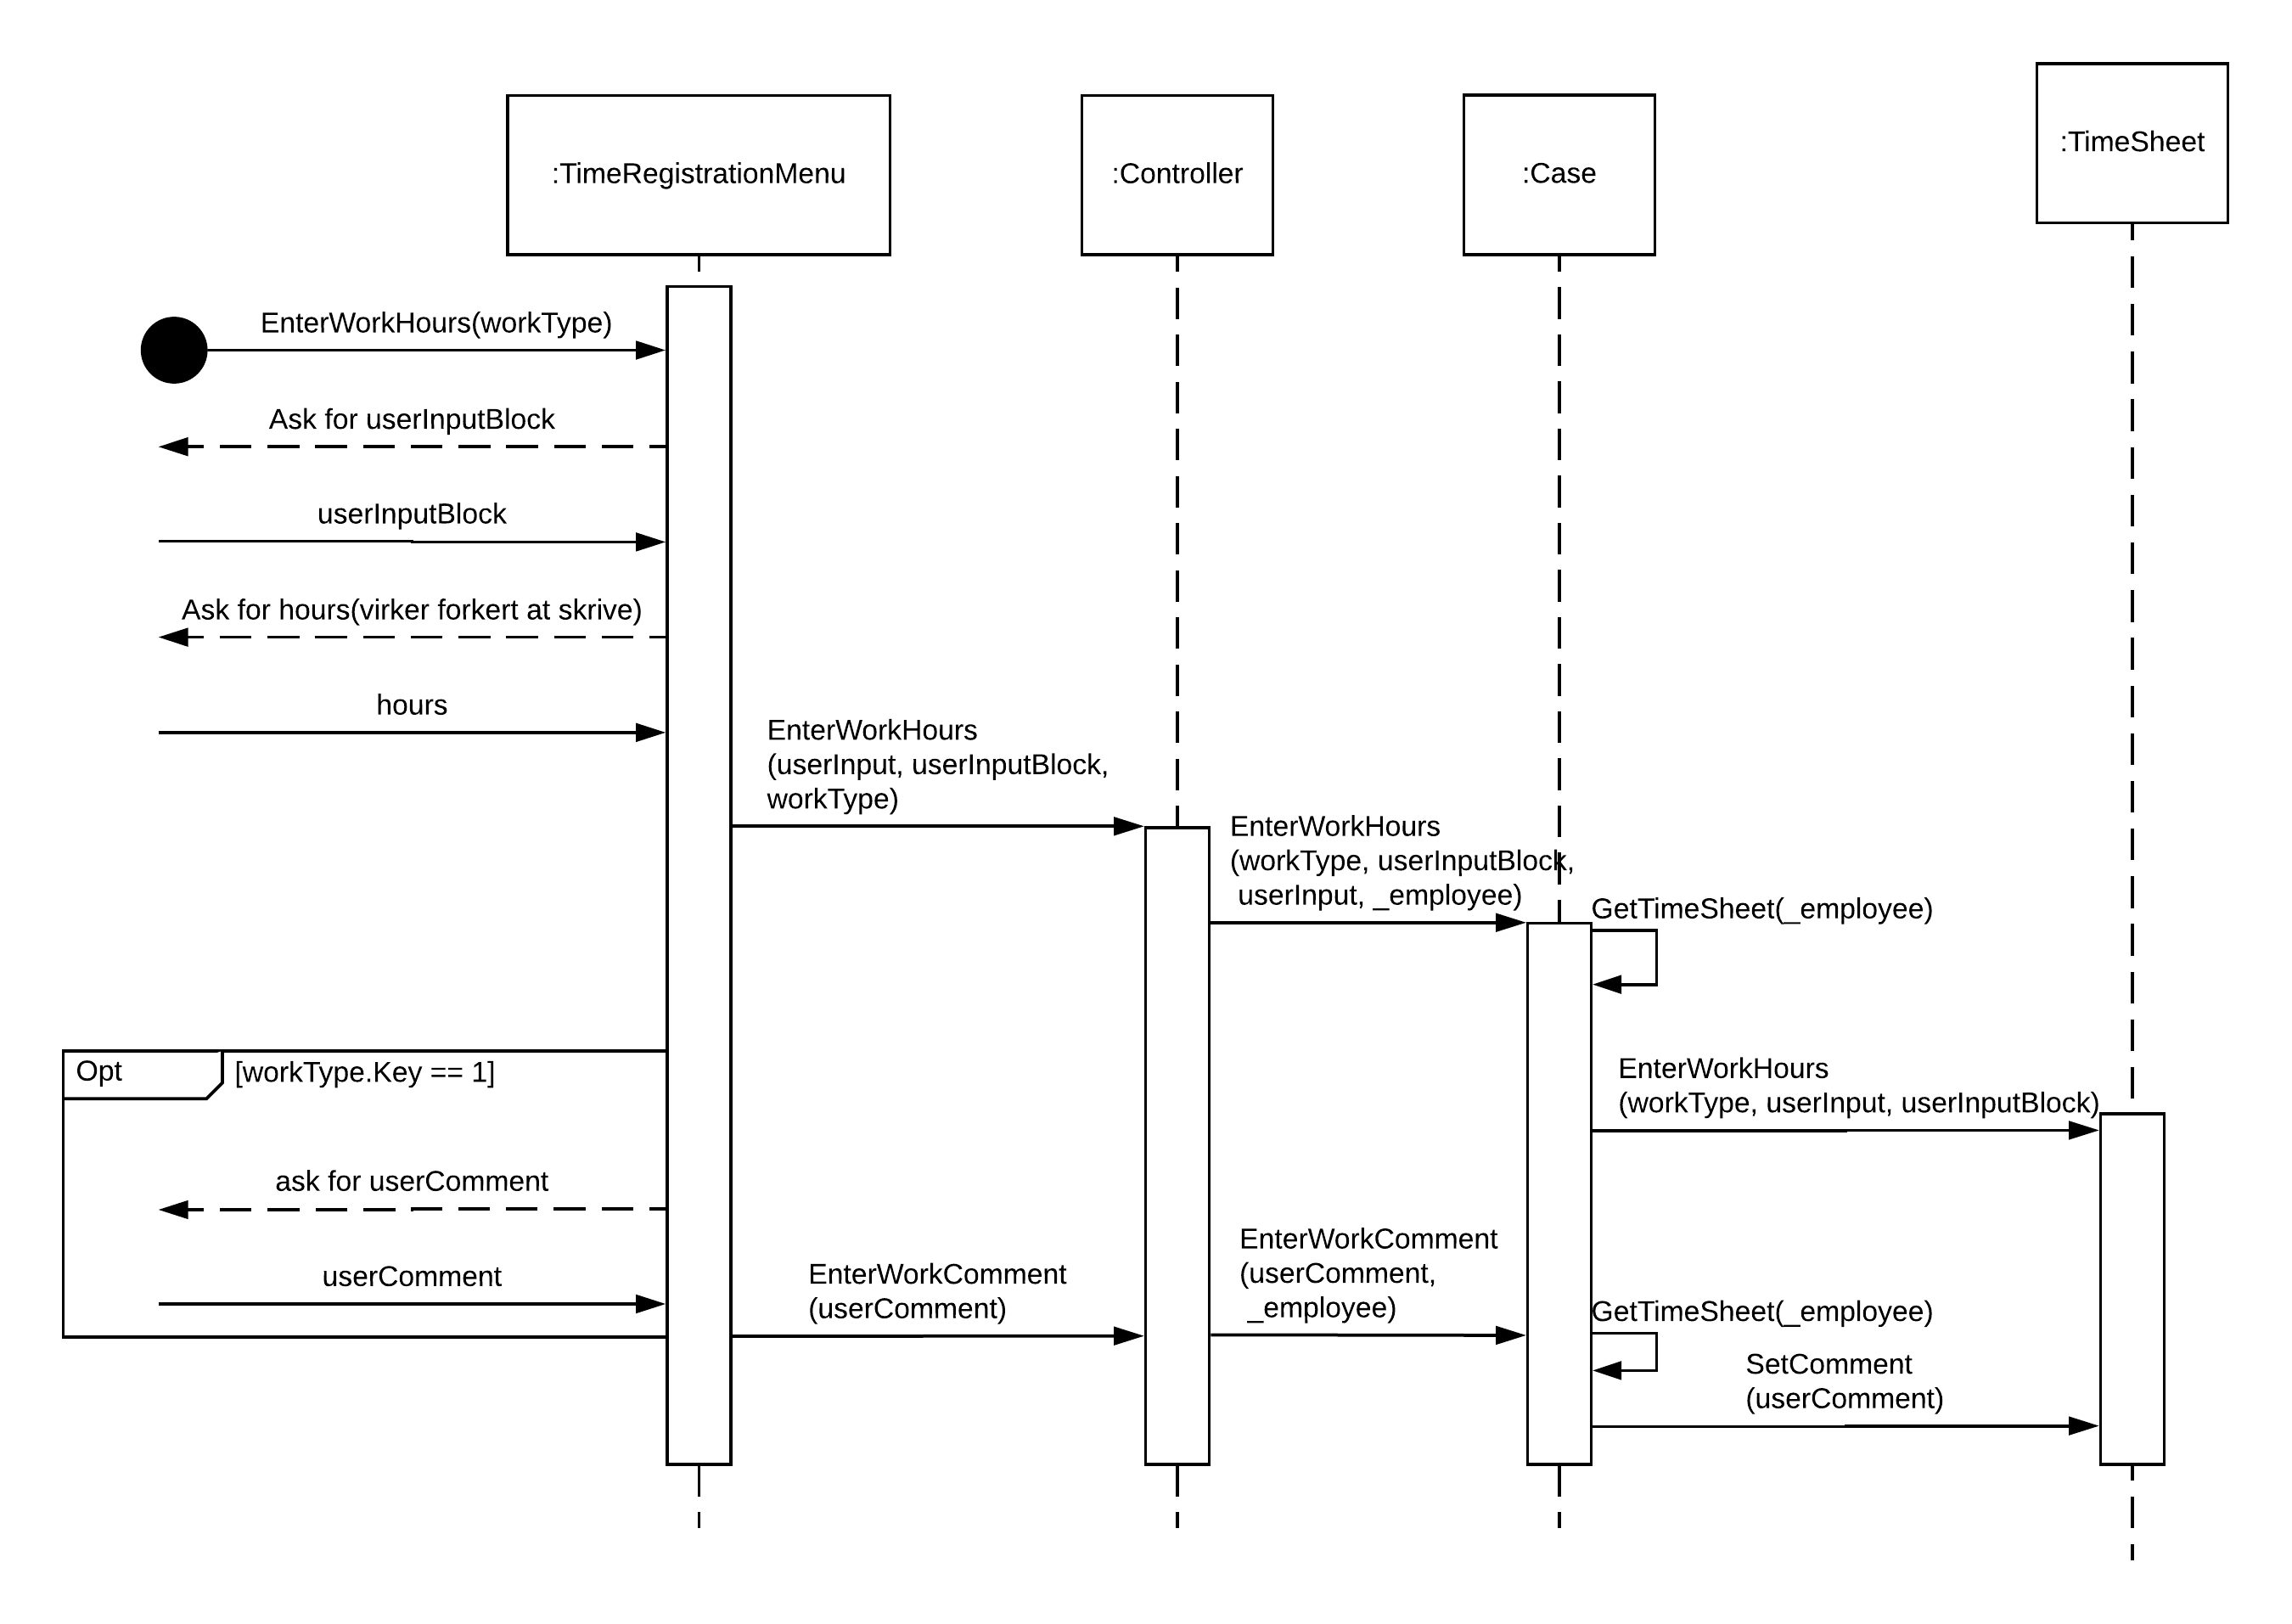
\includegraphics[scale = .6]{SDEnterWorkHours.png}
    \caption{SD for EnterWorkHours metoden.}
    \label{fig:SDEnterWorkHours}
\end{sidewaysfigure}

\subsection{Kode modellering}

Som det kan ses på figur \ref{fig:SDEnterWorkHours} kalder timeregistreringsmenuobjektet controllens EnterWorkHours metode.

\begin{figure}[H]
    \makebox[\textwidth][c]{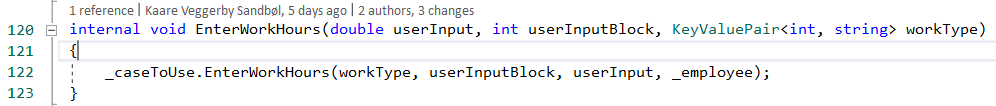
\includegraphics[scale = .8]{ControllerEnterWorkHours.png}}
    \caption{Kodeuddrag for controllerens EnterWorkHours metode}
    \label{fig:SDEnterWorkHours}
\end{figure}


